\section{Reconstruction}\label{sec:recon}

Table~\ref{tab:recon} and Figure~\ref{fig:recon} (left) report explained variance for the 108 base SAEs on the
held-out OWT test split (\evlabel{test}). Reconstruction degrades with depth for every architecture: EV is 0.88--0.95 at
layers 0--2 for the matched runs and falls to 0.757 (ReLU) and 0.815 (TopK and JumpReLU) at layer 11. Seed standard
deviations are at most 0.002 apart from the unmatched layer-0 JumpReLU run.

The best architecture depends on the layer. Compared pairwise by seed, ReLU reconstructs best at layer 1, ReLU and
JumpReLU tie at layer 2, JumpReLU is best at layers 3--9, and JumpReLU and TopK are approximately equal at layers
10--11. No architecture wins at every layer, and at layers 1--11 the spread between architectures (at most about 0.06
EV) is smaller than the loss each architecture suffers between layer 1 and layer 11 (0.11--0.18 EV).

One qualification matters for everything that follows. Sparsity is matched on OWT, but not on task prompts: on
Geometry of Truth final tokens TopK always uses 128 latents, whereas ReLU uses 32--110 and JumpReLU 23--92 at layers
1--11. Architecture differences in information preservation are therefore confounded with task-level sparsity, and we
do not rank architectures on them.

% generated by scripts/shared/build_paper_artifacts.py from results/openwebtext/reconstruction_evaluation/uninterrupted_protocol/all_layers_summary.csv
\begin{table}[t]
\centering
\small
\caption{Reconstruction on the OWT test split (TEST; 12{,}700 tokens), width 3072, target L0 = 128. Layer-0 JumpReLU includes the unmatched seed 42 (L0 73.6). Source: \texttt{results/openwebtext/reconstruction\_evaluation/uninterrupted\_protocol/all\_layers\_summary.csv}.}
\label{tab:recon}
\begin{adjustbox}{max width=\linewidth}
\begin{tabular}{rcccccc}
\toprule
Layer & \multicolumn{3}{c}{OWT test EV (mean$\pm$sd, 3 seeds)} & \multicolumn{3}{c}{OWT test L0} \\
\cmidrule(lr){2-4}\cmidrule(lr){5-7}
 & ReLU & TopK & JumpReLU & ReLU & TopK & JumpReLU \\
\midrule
0 & 0.950$\pm$0.000 & 0.911$\pm$0.000 & 0.826$\pm$0.101 & 135.1 & 125.3 & 110.3 \\
1 & 0.937$\pm$0.000 & 0.921$\pm$0.001 & 0.933$\pm$0.000 & 132.2 & 128.0 & 129.3 \\
2 & 0.936$\pm$0.000 & 0.926$\pm$0.000 & 0.935$\pm$0.002 & 131.9 & 128.0 & 129.0 \\
3 & 0.905$\pm$0.000 & 0.906$\pm$0.000 & 0.915$\pm$0.001 & 131.7 & 128.0 & 129.1 \\
4 & 0.872$\pm$0.000 & 0.884$\pm$0.000 & 0.893$\pm$0.001 & 131.1 & 128.0 & 129.1 \\
5 & 0.848$\pm$0.000 & 0.868$\pm$0.000 & 0.875$\pm$0.000 & 130.8 & 128.0 & 129.0 \\
6 & 0.832$\pm$0.001 & 0.857$\pm$0.000 & 0.865$\pm$0.000 & 131.0 & 128.0 & 129.1 \\
7 & 0.819$\pm$0.001 & 0.850$\pm$0.000 & 0.855$\pm$0.000 & 131.4 & 128.0 & 129.9 \\
8 & 0.805$\pm$0.000 & 0.840$\pm$0.000 & 0.844$\pm$0.000 & 131.9 & 128.0 & 130.3 \\
9 & 0.789$\pm$0.001 & 0.831$\pm$0.000 & 0.833$\pm$0.000 & 132.4 & 128.0 & 131.0 \\
10 & 0.773$\pm$0.000 & 0.822$\pm$0.000 & 0.823$\pm$0.000 & 132.7 & 128.0 & 131.6 \\
11 & 0.757$\pm$0.001 & 0.815$\pm$0.000 & 0.815$\pm$0.000 & 133.2 & 128.0 & 132.1 \\
\bottomrule
\end{tabular}
\end{adjustbox}
\end{table}


\begin{figure}[t]
  \centering
  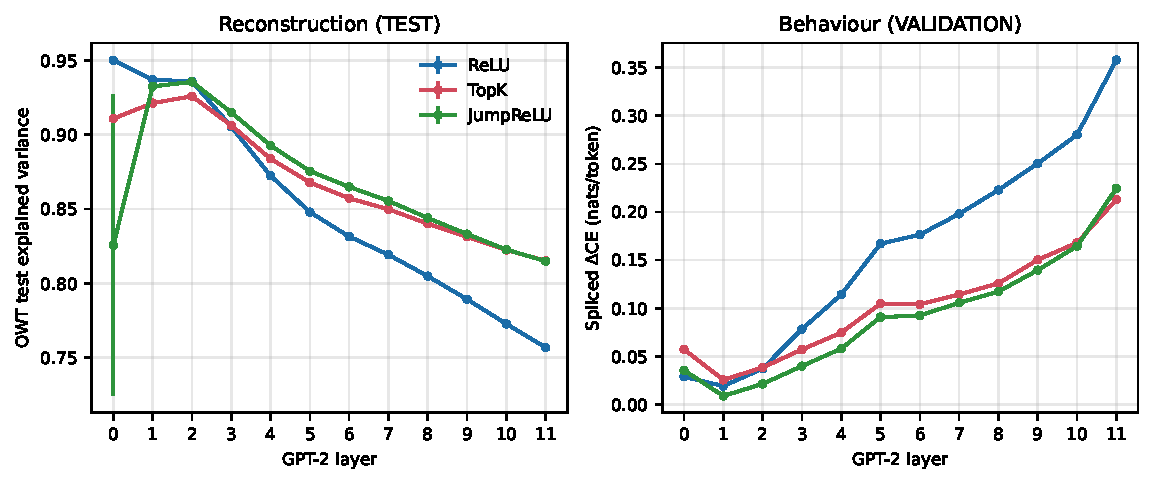
\includegraphics[width=\linewidth]{fig_reconstruction_behaviour}
  \caption{GPT-2 Small reconstruction and behaviour by layer for the 108 base SAEs. Left: OWT test explained
  variance (\evlabel{test}; error bars are seed standard deviations). Right: increase in next-token cross-entropy when
  the reconstruction is spliced into the model (\evlabel{validation}).}
  \label{fig:recon}
\end{figure}
